\documentclass[tikz, border=4pt]{standalone}
\usepackage{tikz}
\usepackage{physics}
\usepackage{siunitx}
\usepackage{ifthen}
\usepackage{tikz}
\usepackage[outline]{contour}
\usepackage{silence}

\usetikzlibrary{calc}
\usetikzlibrary{angles,quotes}
\usetikzlibrary{arrows.meta}
\usetikzlibrary{patterns}

\AtBeginDocument{\RenewCommandCopy\qty\SI}
\tikzset{>=latex}
\contourlength{1.4pt}

% -----------------------------------------------------------------------------
% Color palette
% -----------------------------------------------------------------------------
\colorlet{angleColor}{blue!70!black}
\colorlet{forceColor}{red!65!black}
\colorlet{forceComponentColor}{red!50!blue!80!black!80}
\colorlet{sensorTrackColor}{black!50}
\colorlet{signalOutputColor}{green!70!black}
\colorlet{supplyTerminalColor}{red!70!black}
\colorlet{groundTerminalColor}{blue!70!black}
% \colorlet{uColor}{green!50!black};
% \colorlet{omegaColor}{orange!90!black};
% \colorlet{tauColor}{green!80!black};

% -----------------------------------------------------------------------------
% Reusable drawing styles (used by pendulum.tex)
% -----------------------------------------------------------------------------
\tikzset{
  supportSurface/.style={
    preaction={fill,top color=black!10,bottom color=black!5,shading angle=20},
    fill,
    pattern=north east lines,
    draw=none,
    minimum width=0.3,
    minimum height=0.6
  },
  forceVector/.style={
    ->,
    forceColor,
    very thick,
    line cap=round
  },
  information text/.style={
    rounded corners,
    fill=red!10,
    inner sep=1ex
  }
}

\usetikzlibrary{arrows.meta,patterns}

% =============================================================================
% Coordinate system pic (for pendulum hinge)
% =============================================================================
\tikzset{
  coordsys/.pic={
      \fill[red] (0,0) circle(0.05);
      \draw[->,thick, red] (0,0) -- (1,0) node[right] {$e_x$};
      \draw[->,thick, red] (0,0) -- (0,1) node[above] {$e_y$};
    }
}

\begin{document}
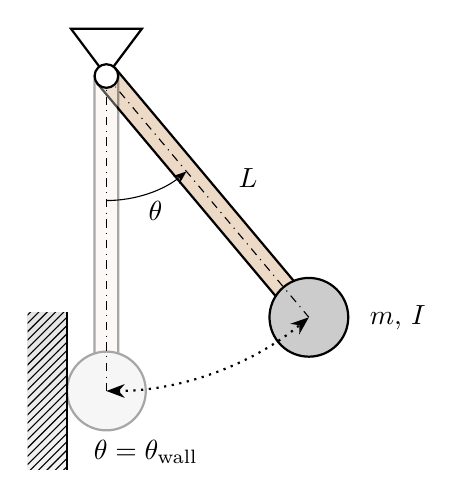
\begin{tikzpicture}[scale=1.0, >=Stealth]
\def\L{4}       % rod length
\def\W{0.3}     % rod width
\def\R{0.5}     % pendulum head radius
\def\ang{40}    % angle from negative y-axis (hanging down)
\def\F{0.9}     % force arrow extension beyond bob
\def\wallW{0.5} % wall thickness
\def\wallH{2}   % wall height

\coordinate (O) at (0,0);

% Pendulum rod (rectangle, rotated about hinge)
\begin{scope}[rotate=\ang, transparency group]
  % Pendulum rod
  \draw[thick, fill=brown!30] (-\W/2,0) rectangle (\W/2,-\L);
  
  % Pendulum head (circle at end of rod)
  \draw[thick, fill=gray!40] (0,-\L) circle(\R);
  \node[right=\R+18pt] at (0,-\L) {$m,\,I$};

  % Pendulum center line
  \draw[dash dot, thin] (0,0) -- (0, -\L);
  
\end{scope}

% === Ghost pendulum at theta = 0 ===
\begin{scope}[rotate=0, transparency group, opacity=0.35]
  \draw[thick, fill=brown!15] (-\W/2,0) rectangle (\W/2,-\L);
  \draw[thick, fill=gray!20] (0,-\L) circle(\R);
\end{scope}

% Vertical reference line (theta = 0)
\draw[dash dot, thin] (0,0) -- (0,-\L);

% Pendulum trajectory arc (full oscillation range)
\draw[<->, dotted, thick] (-90:\L) arc (-90:-90+\ang:\L);

% Wall (impact surface at theta = 0, right edge at x = -R)
\draw[supportSurface] (-\R-\wallW, -\L-\wallH/2) rectangle (-\R, -\L+\wallH/2);
\draw[thick] (-\R, -\L-\wallH/2) -- (-\R, -\L+\wallH/2);

% === Forces at pendulum head ===
\coordinate (M) at (\ang-90:\L);

% Angle theta at hinge (between vertical and rod midline)
\coordinate (B) at (0,-1.5);
\draw pic[->,"$\theta$", draw, angle radius=45, angle eccentricity=1.15] {angle=B--O--M};

% Length L annotation
\node at (1.8, -1.3) {$L$};

\node[below] at (\R, -\L-\R) {$\theta = \theta_\text{wall}$};

% Revolute joint: classical triangle + small circle
\draw[thick, fill=white] (-0.45,0.6) -- (0.45,0.6) -- (0,0) -- cycle;
\draw[thick, fill=white] (O) circle(\W/2);

% --- Interface anchors (for wiring in assembly) ---
\coordinate (pend-tau)   at (0, 0);     % torque input
\coordinate (pend-theta) at (0, 0);     % angle output (same shaft)

\end{tikzpicture}

\end{document}
